\chapter{Yara Rules}
\newpage

\section{lecture}
\textbf{YARA Overview}

YARA is a widely used and powerful tool for identifying and classifying files or data based on patterns, rules, or signatures. It is particularly valuable in cybersecurity and malware analysis.

\textbf{Core Components}
\begin{itemize}
    \item \textbf{Pattern Matching}
        \begin{itemize}
            \item Text and binary pattern detection
            \item File content analysis
            \item Memory stream scanning
            \item Real-time content monitoring
        \end{itemize}

    \item \textbf{Rules System}
        \begin{itemize}
            \item Custom pattern definition
            \item Condition specification
            \item Metadata integration
            \item YARA-specific syntax
        \end{itemize}

    \item \textbf{Usage Applications}
        \begin{itemize}
            \item Malware detection
            \item Virus identification
            \item Threat classification
            \item Data categorization
            \item Content identification
        \end{itemize}

    \item \textbf{Extensibility Features}
        \begin{itemize}
            \item Custom rule creation
            \item Community rule sharing
            \item Rule modification capabilities
            \item Module expansion options
        \end{itemize}

    \item \textbf{Implementation Tools}
        \begin{itemize}
            \item Command-line interface
            \item Integration libraries
            \item Software integration capabilities
            \item Automation support
        \end{itemize}
\end{itemize}

\textbf{Summary}
YARA serves as a versatile security tool that enables threat detection and content classification through user-defined pattern matching rules and behavioral analysis capabilities.

\subsubsection{BAsics of YARA Rules}
\begin{itemize}
  \item Identifying malware: hash code
  \begin{itemize}
    \item Problem: very restrictive
    \item change one bit $\rightarrow$ different hash code
  \end{itemize}
  \item Alternative
  \begin{itemize}
    \item identify marker patterns
    \item Standard: YARA rules
    \item Yet Another Recursive/Ridiculous Acronym
  \end{itemize}
\end{itemize}

\textbf{Yara By Example}

Yes, there's a YARA language specification for listings. It can be enabled by using:

\begin{lstlisting}[language=YARA]
rule macrocheck : maldoc {
    meta:
        Author = "Fireeye Labs"
        Description = "Identify office documents with the MACROCHECK credential stealer in them..."
        Reference = "https://www.fireeye.com/blog/threat-research/2014/11/fin4_stealing_insid.html"
    
    strings:
        $PARAMpword = "pword=" ascii wide
        $PARAMmsg = "msg=" ascii wide
        $PARAMuname = "uname=" ascii
        $userform = "UserForm" ascii wide
        $userloginform = "UserLoginForm" ascii wide
        $invalid = "Invalid username or password" ascii wide
        $up1 = "uploadPOST" ascii wide
        $up2 = "postUpload" ascii wide
    
    condition:
        all of ($PARAM*) or 
        (
            ($invalid or $userloginform or $userform) and 
            ($up1 or $up2)
        )
}
\end{lstlisting}

\begin{center}
  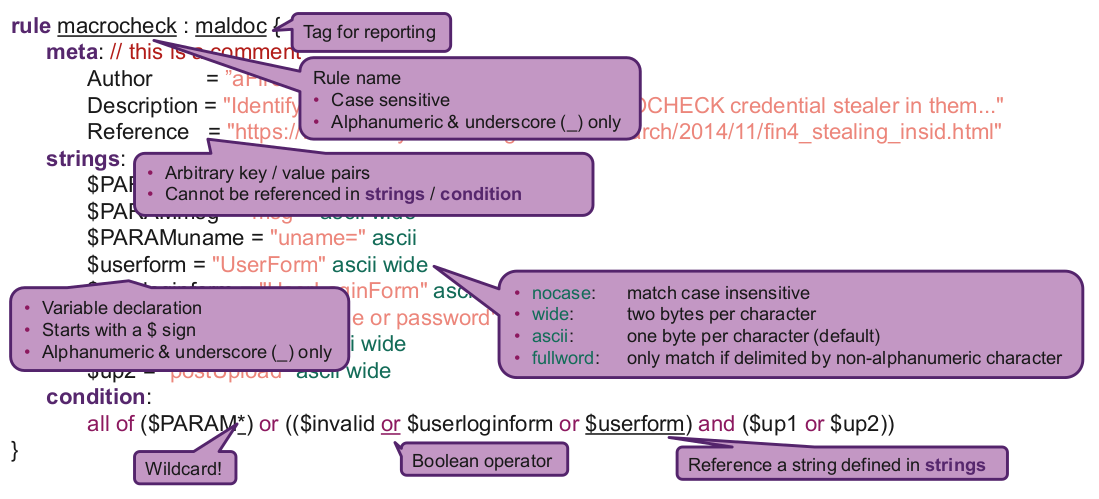
\includegraphics[width=\textwidth]{resources/08-yara-rules-example.png}
\end{center}
\textbf{More examples}

\begin{lstlisting}[language=YARA]
  meta: ...
    strings:
    $a1 = { 64 8B (05|0D|15|1D|25|2D|35|3D) 30 00 00 00 }
    $a2 = {64 A1 30 00 00 00}
    $a3 = {FF 75 ?? FF 55 ?? A?}
    $a4 = {68 [-3] 07 00 [1-5] FF 15}
  condition:
    3 of them
    and for any i in (1 .. #a3): (uint8(@a3[i] + 2) == uint8(@a3[i] + 5))
    and !a4 > 100
\end{lstlisting}

\begin{lstlisting}[language=YARA]
  private rule WindowsPE {
    strings:
      $mz = { 4D 5A }
    condition:
      $mz at 0 and filesize < 250KB and uint32(uint32(0x3C)) == 0x00004550
  }
  rule bar {
    meta: ...
    strings:
      $re = /bn1=.{32}&sk1=[0-9a-zA-Z]{32}/
    condition:
      WindowsPE and $re
  }
\end{lstlisting}

\textbf{Hex Strings}
\begin{lstlisting}[language=YARA]
rule hex_example {
    strings:
        $hex1 = { 4D 5A 90 00 03 }
        $hex2 = { 4? 5A ?? 00 }    \/\/ with wildcards
}
\end{lstlisting}

\textbf{Text Strings}
\begin{lstlisting}[language=YARA]
rule text_example {
    strings:
        $text1 = "malicious string"
        $text2 = "another string"
}
\end{lstlisting}

\textbf{Case Insensitive}
\begin{lstlisting}[language=YARA]
rule case_insensitive {
    strings:
        $str = "MaLiCiOuS" nocase
        $str2 = "Password" nocase ascii
}
\end{lstlisting}

\textbf{Wide Characters}
\begin{lstlisting}[language=YARA]
rule wide_chars {
    strings:
        $w1 = "Admin" wide
        $w2 = "Login" ascii wide  \/\/ matches both
}
\end{lstlisting}

\textbf{XOR Strings}
\begin{lstlisting}[language=YARA]
rule xor_example {
    strings:
        $xor = "Secret" xor
        $xor_range = "Admin" xor(1-255)  \/\/ specific range
}
\end{lstlisting}

\textbf{Base64 Strings}
\begin{lstlisting}[language=YARA]
rule base64_example {
    strings:
        $b64 = "Password" base64
        $b64wide = "Admin" base64wide
}
\end{lstlisting}

\textbf{Private Strings}
\begin{lstlisting}[language=YARA]
private rule private_example {
    strings:
        $priv = "Internal String"
    condition:
        $priv
}
\end{lstlisting}

\subsubitem{PACKERS}
\begin{itemize}
  \item • Most malware today is packed in some way to help get around AV signature detection
  \item There are over 8000 known packers out there, each with their own signatures.
  \item They can range from simple compression to full on encryption / debugger detection and generally make the life of the Malware Reverser a pain.
  \item Packers are not fool proof - the exe HAS to be decrypted / decompressed at SOME point in order to run on the OS.
\end{itemize}

\subsection{How To Use YARA Rules}
\textbf{File System Scan}
\begin{lstlisting}[language=bash]
  yara -r /opt/applic/yara-rules/index.yar /home/hacker/malware-samples
  yara -w -r -t Packer -t Compiler /opt/applic/yara-rules/index.yar /home/hacker/malware-samples
\end{lstlisting}
\begin{itemize}
  \item[-r] recursively
  \item[-w] suppress warnings
  \item[-t] search for tags
\end{itemize}

\textbf{Volatility \& YARA Examples}

\textit{Volatility2}
\begin{lstlisting}[language=bash]
volatility2 -f ./0zapftis.vmem yarascan -y /opt/applic/yara-rules/malware/MALW_LuaBot.yar
volatility2 -f ./0zapftis.vmem yarascan --yara-file /opt/applic/yara-rules/malware/MALW_LuaBot.yar
volatility2 -f ./0zapftis.vmem yarascan --yara-rule "http:"
\end{lstlisting}

\textit{Volatility3}
\begin{lstlisting}[language=bash]
volatility3 -f ./0zapftis.vmem yarascan.YaraScan --yara-rules "http:"
volatility3 -f /home/hacker/Downloads/0zapftis.vmem windows.vadyarascan.VadYaraScan --yara-file ./packers_index.yar
volatility3 -f /home/hacker/Downloads/0zapftis.vmem yarascan.YaraScan --yara-file ./packers_index.yar
\end{lstlisting}

\subsection{File Extraction from Network Dump (PCAP)}
\begin{itemize}
  \item foremost -t all -f tcpdump.pcap
  \item binwalk -e tcpdump.pcap
  \item tcpflow -r tcpdump.pcap -o .
  \item chaosreader tcpdump.pcap
  \item Wireshark – Follow TcpStream -> SaveAs ...
\end{itemize}


\section{exercise}
